\newpage


\section{Lazy Code Motion}

In 1979, Morel and Renvoise came up with an exciting new technique,
the suppression of partial redundancies \cite{morel1979global}. Their technique
uniformly subsumed loop invariant code motion, common
subexpression elimination, and the elimination of redundant
computations. Probably, the most appealing facet of their
technique was its structural purity: the transformation was
solely based on data-flow analysis and did not require any
specific knowledge on the control flow of the programs under investigation. On the other hand, their genuine proposal
was conceptually complex. It involved an equation system
of four highly interacting global properties while still suffering from three deficiencies. First, too few partial redundancies are removed. Intuitively, this was due to Morel’s and
Renvoise’s design decision to insert code at the nodes of the
underlying flow graph rather than at its edges, which unnecessarily restricted the possible computation points. Second,
code was moved too far, which led to unnecessary register
pressure. And third, the node placement was based on bidirectional data-flow equations which — from a conceptual
point of view — are difficult to comprehend and — from a
computational point of view — are more costly to compute.

As we started our work on lazy code motion, we were convinced that research efforts based on modifying the Morel/-
Renvoise-style equations had led into a dead end. Partial redundancy elimination (PRE) is a beautiful technique with
a simple underlying basic idea: expressions are hoisted to
earlier program points increasing thereby their potential to
make the original ones fully redundant, which can then be
eliminated. We had the strong belief that it must be possible to construct a PRE-technique which is solely composed
out of simple and well-understood components.

\textit{Decomposing the problem.} A key idea to attack the problem was its \textbf{decomposition} based on a clean separation of
concerns. We noticed that there are two optimization goals
with a natural hierachy: the primary is to reduce the number of computations to a minimum (computational optimality); 
the secondary to avoid unnecessary code movement to
\textbf{minimize the lifetimes of temporaries and hence the register
pressure (lifetime optimality)}. There is no a topological order for the bidirectional dataflow analysis, so this does complicate things.

\textit{Solving the problem.} Fortunately, we already had an offthe-shelf solution for the first optimization goal. Investigating the relationship between model checking and data-flow
analysis has led to a modal logic specification of a computationally optimal PRE following an as-early-as-possible code
placement strategy \cite{steffen1991data}. We called the resulting transformation “Busy Code Motion (BCM),” as it hoists code as
far as possible. Technically it required only two simple unidirectional data-flow analyses. This simplicity revealed the
solution to our secondary goal, the avoidance of unnecessary code motion: the code only had to “sink back” from
the BCM insertion points as far as computational optimality was preserved, which can be realized simply by adding another 
unidirectional data-flow analysis. The resulting transformation, which \textbf{solves the problem of unnecessary register
pressure}, hoists code just far enough to ensure computationally optimal results, the reason for it being called “Lazy
Code Motion (LCM).”

This successful way of playing with simple analysis components was later extended to also control/minimize code
size \cite{ruthing2000sparse}. Here, the natural trade-off between the optimization goals led to different solutions depending on the chosen
priority between size and speed.


\subsection{Big Picture}

First calculates the “earliest” set of blocks for insertion, this maximizes redundancy elimination but may also result in long register lifetimes.
Then it calculates the “latest” set of blocks for insertion, this achieves the same amount of redundancy elimination as “earliest” but hopefully reduces register lifetimes


\subsection{PRE vs. LCM}


The goal of PRE is that by {\color{red}moving around} the places where an expression is
evaluated and keeping the result in a temporary variable when
necessary, we often can {\color{red}reduce the number of evaluations} of this
expression along many of the execution paths, {\color{red}while not
increasing that number along any path.} However, it is {\color{red}not} possible to eliminate all redundant computations along
every path, unless we are allowed to {\color{red}change the control flow
graph} by {\color{red}creating new blocks} and {\color{red}duplicating blocks.}

\begin{definition}{New blocks creation}
    It can be used to break {\color{red}“critical edge”},
    which is an edge leading from a node with more than one
    successor to a node with more than one predecessor.
    \begin{figure}[H]
        \centering
         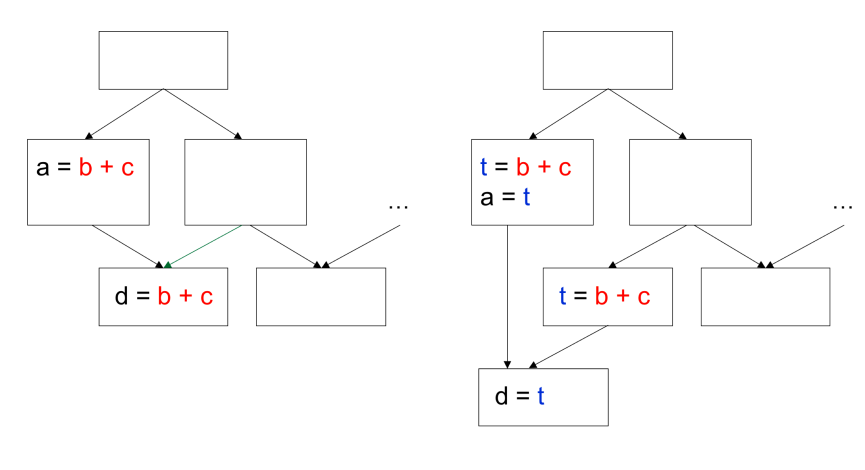
\includegraphics[width=0.5\textwidth]{p104.png}
             \caption{Example of new block creation}
             \label{fig:p104}
    \end{figure}

\end{definition}

\begin{definition}{Block duplication}
    It can be used to isolate the path where
    redundancy is found.
    \begin{figure}[H]
        \centering
         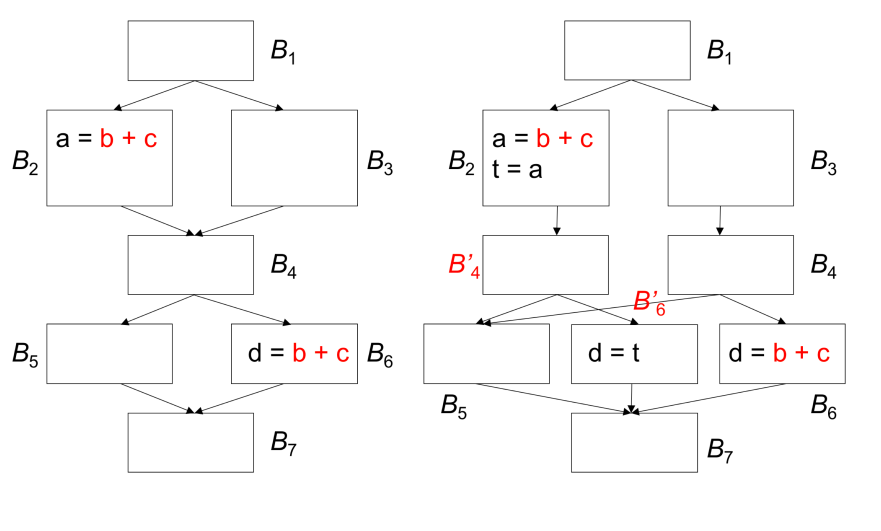
\includegraphics[width=0.5\textwidth]{p105.png}
             \caption{Example of block duplication}
             \label{fig:p105}
    \end{figure}

\end{definition}


\subsection{Preprocessing: Preparing the Flow Graph}

First, we need modify the flow graph. Inorder to ensure redundancy elimination power, we add
a basic block for every edge that leads to a basic block with multiple
predecessors. Also, in LCM, we restrict placement of instructions to the beginning of a basic block
Consider each statement as its own basic block to keep algorithm simple.


\begin{definition}{Full Redundancy: A Cut Set in a Graph}
    Full redundancy at p: expression a+b redundant on all paths
    \begin{itemize}
    \item a cut set: nodes that separate entry from p (could have multiple cut sets).
    \item each node in a cut set contains a calculation of a+b.
    \item a, b not redefined.
    \end{itemize}

    \begin{figure}[H]
        \centering
         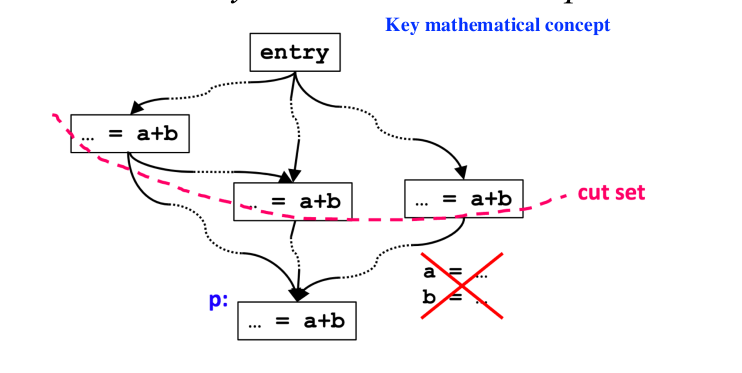
\includegraphics[width=0.5\textwidth]{p106.png}
             \caption{Full Redundancy}
             \label{fig:p106}
    \end{figure}
\end{definition}


\begin{definition}{Partial Redundancy: Completing a Cut Set}

    Partial redundancy at p: redundant on some but not all paths

    \begin{itemize}
        \item Add operations to create a cut set containing a+b
        \item Note: Moving operations up can eliminate redundancy
    \end{itemize}

    \begin{figure}[H]
        \centering
         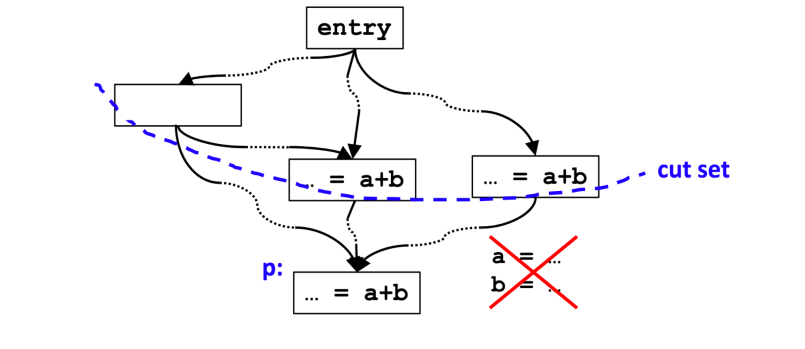
\includegraphics[width=0.5\textwidth]{p107.png}
             \caption{Partial Redundancy}
             \label{fig:p107}
    \end{figure}
\end{definition}



\subsection{Pass 1: Anticipated Expression}


\begin{center}
    \begin{tabular}{|c|c|}
   \hline Direction & Backword\\
   \hline Domain & Set of expressions\\
   \hline Meet operator & \( \cap \)\\
   \hline Boundary & $IN[EXIT] = \phi$ \\  
   \hline Initialization for internal nodes & \( IN[B] = \{ all expressions\} \) \\
   \hline Finited escending chain? &\checkmark  \\
   \hline Transferfunction  & \( f_b(x) = EUse_b \cup (x - EKill_b) \)\\
   \hline Monotone\&Distributive?  & \checkmark \\
   \hline \( EUse_b \) & set of expressions computed in B (EUse, UEEXP). \\
   \hline \( EKill_b \) &set of expressions any of whose operands are defined in B \\
   \hline
   \end{tabular}  
   \end{center}



\subsection{Where to insert/move instructions?}

\subsubsection{Choice 1 : frontier of anticipation}




What is the result if we insert t = a + b at the frontier of anticipation ?
i.e., those BBs for which a + b is anticipated to the entry of BB, but not anticipated
to the entry of its parents.?


\begin{figure}[H]
    \centering
     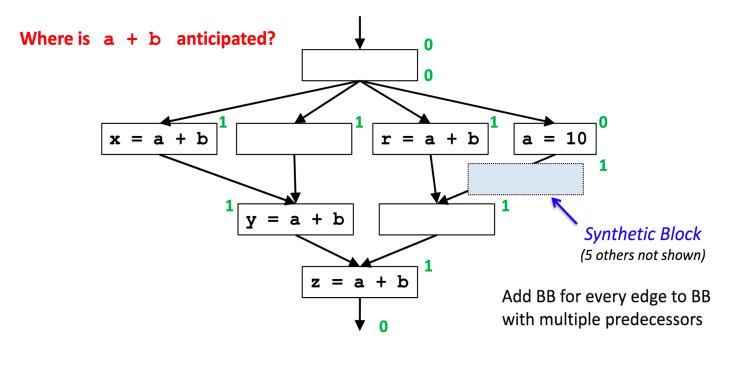
\includegraphics[width=0.8\textwidth]{p110.png}
         \caption{Frontier may be good for this example.}
         \label{fig:p110}
\end{figure}

\begin{figure}[H]
    \centering
     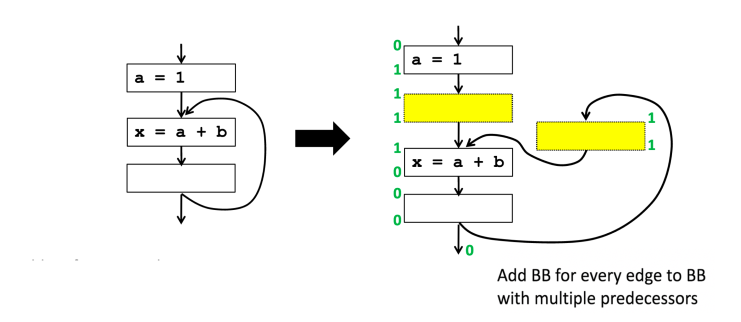
\includegraphics[width=0.8\textwidth]{p108.png}
         \caption{Frontier are clolored in yellow. Frontier of anticipation may be not a good choice. For this example, 
         if we insert t = a + b at the frontier of anticipation, this doesn't eliminate redundancy within loop!}
         \label{fig:p108}
\end{figure}



\begin{figure}[H]
    \centering
     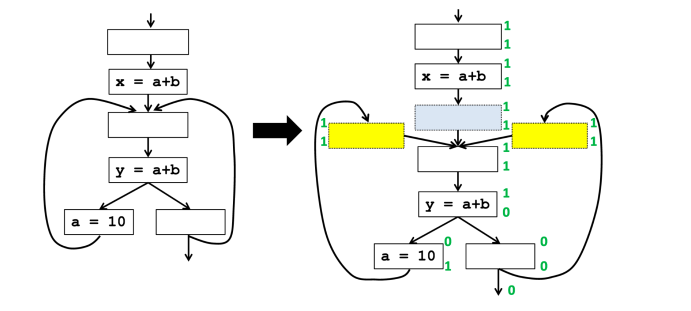
\includegraphics[width=0.8\textwidth]{p109.png}
         \caption{This example can also illustrate frontier is not our choice. In fact, we ideally like to insert “a+b” in this case to the left BB.}
         \label{fig:p109}
\end{figure}


How to find such anticipated frontier and exclude “those not
needed blocks” discussed in previous loop examples? Our final solution: 
Place expression at “anticipated” but not “will be
available” blocks

\subsection{Pass 2: Place As Early As Possible}


\begin{center}
    \begin{tabular}{|c|c|}
   \hline Name & Available Expressions\\    
   \hline Direction & Forward\\
   \hline Transferfunction  & \( f_b(x) = (Anticipated[b].in \cup x ) - EKill_b \)\\
   \hline Domain & Set of expressions\\
   \hline Meet operator & \( \cap \)\\
   \hline Boundary & $OUT[Entry] = \phi$ \\  
   \hline Initialization for internal nodes & \( OUT[B] = \{ all expressions\} \) \\
   \hline
   \end{tabular}  
   \end{center}


   \[
     \mathrm{earliest[b] = anticipated[b] - available[b]}
   \]


   \subsection{Pass 3: Lazy Code Motion}
The values of expressions found to be redundant are usually
held in registers until they are used. Computing a value as late as possible minimizes its lifetime:
the duration between the time the value is defined and the
time it is last used. Minimizing the lifetime of a value in turn minimizes the usage of
a register. 


\begin{definition}{postponable}

    An expression e is postponable at a program point p if
    \begin{itemize}
    \item all paths leading to p have seen earliest placement of e
    \item but not a subsequent use
    \end{itemize}

    \begin{figure}[H]
        \centering
         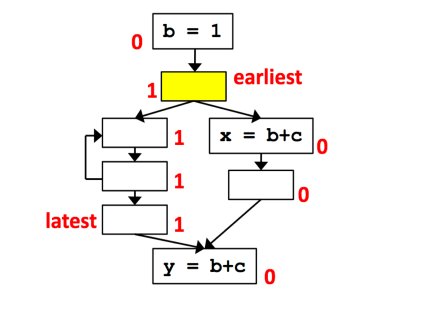
\includegraphics[width=0.6\textwidth]{p111.png}
             \caption{An example to illustrate Postponable Expressions.}
             \label{fig:p111}
    \end{figure}
\end{definition}




    \begin{center}
        \begin{tabular}{|c|c|}
       \hline Name & Postponable Expressions\\    
       \hline Direction & Forward\\
       \hline Transferfunction  & \( f_b (x) = (earliest[b] \cap x) - EUse_b \)\\
       \hline Domain & Set of expressions\\
       \hline Meet operator & \( \cap \)\\
       \hline Boundary & $OUT[Entry] = \phi$ \\  
       \hline Initialization for internal nodes & \( OUT[B] = \{ all expressions\} \) \\
       \hline
       \end{tabular}  
       \end{center}


       \begin{figure}[H]
        \centering
         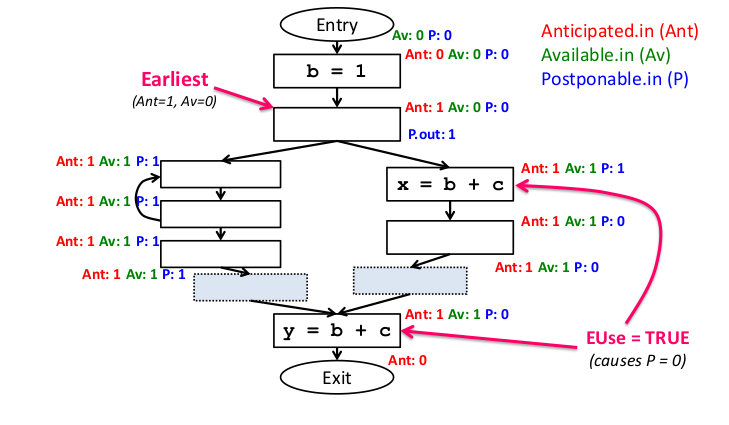
\includegraphics[width=0.6\textwidth]{p112.png}
             \caption{An example to illustrate Postponable.}
             \label{fig:p112}
    \end{figure}

    \begin{figure}[H]
        \centering
         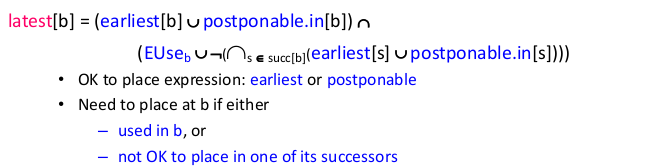
\includegraphics[width=0.6\textwidth]{p113.png}
             \label{fig:p113}
    \end{figure}



    \begin{figure}[H]
        \centering
         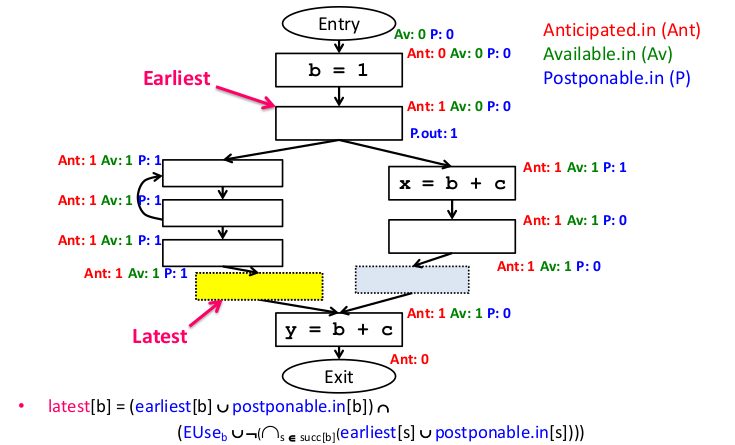
\includegraphics[width=0.6\textwidth]{p114.png}
         \caption{An example to illustrate “Latest”.}
             \label{fig:p114}
    \end{figure}

\subsection{Pass 4: Cleaning Up}



\begin{center}
    \begin{tabular}{|c|c|}
   \hline Name & Used Expressions\\    
   \hline Direction & Backward\\
   \hline Transferfunction  & \( f_b (x) = (EUse[b] \cap x) - latest[b] \)\\
   \hline Domain & Set of expressions\\
   \hline Meet operator & \( \cup \)\\
   \hline Boundary & $in[exit] = \phi$ \\  
   \hline Initialization for internal nodes & \( in[b] = \phi \)  \\
   \hline
   \end{tabular}  
   \end{center}


   For all basic blocks b, if (x+y) $\in$ (latest[b] $\cap$ used.out[b]), at beginning of b:
   add new t = x+y, then replace every original x+y by t

% \begin{definition}{Cut Set}
% A cut set are nodes that separate entry from p. a cut set contains calculation of a+b

% \end{definition}



